\documentclass[letterpaper]{article}

% For final submission, replace this generic article setup with:
% \usepackage{aaai}
\usepackage{times}
\usepackage{helvet}
\usepackage{courier}
\usepackage{amsmath,amssymb}
\usepackage{booktabs}
\usepackage{graphicx}
\usepackage{multirow}
\usepackage{xcolor}

\newcommand{\method}{DePose-Fi}

\title{\method: Decomposition-First Wi-Fi Human Pose Estimation with Tiny Machine Learning}

\author{
Toan D. Gian\\
TODO: affiliation\\
\texttt{TODO: email}
}

\begin{document}
\maketitle

\begin{abstract}
Wi-Fi human pose estimation (HPE) recovers body keypoints from channel state information (CSI), enabling privacy-preserving sensing without cameras or wearable devices. Existing Wi-Fi HPE systems commonly feed raw or weakly processed CSI into neural networks, requiring the model to implicitly discover human-relevant signal structure from a heavily mixed wireless measurement. We argue that this is the wrong abstraction for lightweight Wi-Fi HPE: complicated CSI should first be decomposed into physically meaningful components, and only then passed to a predictor. We present \method, a decomposition-first framework that factorizes each CSI frame into compact link, subcarrier, and packet factors, then predicts pose using tiny machine learning regressors. Under the MM-Fi frame-level protocol used by HPE-Li, rank-4 non-negative CP decomposition compresses each CSI frame from 3420 raw values to 508 component features. On the full MM-Fi protocol-3 frame-level split with 320,760 frames, CP components improve lightweight MLP64 PCK$_{20}$ from 44.69\% to 46.24\% and improve ExtraTrees PCK$_{20}$ from 47.27\% to 50.40\% over raw-statistic features. The deployable CP+MLP64 variant uses only 35.9K parameters and about 1.00M FLOPs per frame, far below HPE-Li's reported 1.66M parameters and 2.42G FLOPs. Component ablation further shows that decomposed factors are pose-relevant. These results support a new direction for Wi-Fi HPE: decompose the wireless signal first, then use small, interpretable predictors.
\end{abstract}

\section{Introduction}

\textbf{Motivation.}
Wi-Fi sensing has become an attractive alternative to camera and wearable sensing because it reuses existing wireless infrastructure and preserves visual privacy. Channel state information (CSI) captures how wireless propagation changes across antennas, subcarriers, and time. These changes encode human presence and motion, enabling tasks such as activity recognition, gesture recognition, localization, and human pose estimation (HPE). HPE is especially demanding: instead of predicting a coarse activity class, the system must recover a structured set of body keypoints from an indirect wireless measurement.

\textbf{Existing limitations.}
Most Wi-Fi HPE systems follow an end-to-end neural paradigm. CSI is transformed into amplitude, phase, image-like, or sequence-like inputs, then a neural model is trained to regress keypoints. This has produced strong results, including lightweight architectures such as HPE-Li. However, raw CSI is not a direct observation of human pose. It is a mixture of line-of-sight propagation, static environmental reflections, human-induced reflections, dynamic interference paths, and hardware noise. A direct neural model must therefore solve two problems at once: discover the human-relevant wireless components and map them to keypoints.

This coupling is problematic for tiny deployment. A large network can hide the decomposition inside its learned layers, but a tiny model cannot easily infer physical structure from mixed CSI. Even when the network is accurate, its representation is difficult to interpret. If a model fails, we do not know whether the error comes from poor signal purification, poor pose mapping, or environment-specific shortcuts.

\textbf{Key idea.}
We propose a decomposition-first view of Wi-Fi HPE. Rather than feeding mixed CSI directly into a predictor, we first factorize CSI into compact components. Each component has a link factor, a subcarrier factor, and a packet activation factor. These factors expose how a latent wireless mode appears across antenna links, frequency, and short-time samples. Once this representation is extracted, pose estimation becomes a simpler regression problem.

This view gives rise to three research questions. \textbf{RQ1:} Can compact decomposed CSI components retain enough information for Wi-Fi HPE? \textbf{RQ2:} Can lightweight ML regressors on decomposed components approach neural HPE accuracy? \textbf{RQ3:} Are the decomposed components actually pose-relevant, or are they merely compressed numerical features? The third question is crucial. A decomposition method is scientifically useful only if its components explain downstream behavior. For this reason, we evaluate not only PCK, but also component ablation and factor-mode importance.

Figure~\ref{fig:overview} summarizes the framework. The raw CSI frame is treated as a tensor rather than a flat feature vector. Non-negative tensor decomposition extracts component factors. The concatenated factors are then used by a lightweight machine learning regressor. This makes the pipeline compact and analyzable: components can be visualized, removed, ranked by importance, and evaluated for pose relevance.

\begin{figure*}[t]
\centering
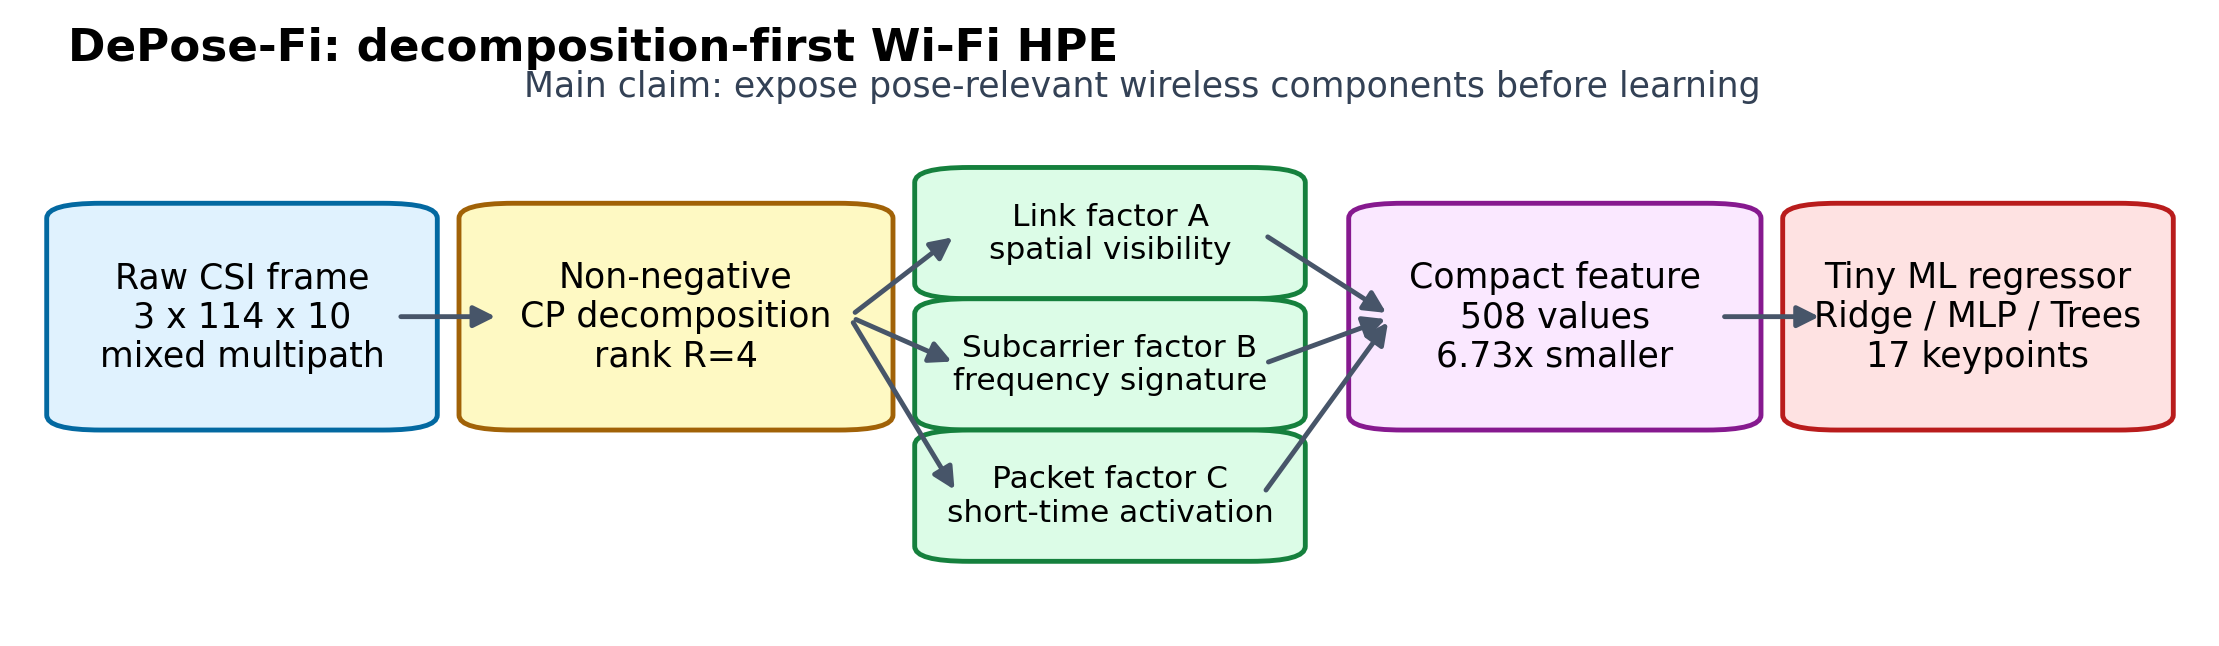
\includegraphics[width=0.95\linewidth]{figures/fig1_overview.pdf}
\caption{Overview of \method. Raw CSI is a mixture of propagation and motion effects. \method\ first decomposes each CSI frame into link, subcarrier, and packet factors, then uses compact component features for lightweight pose regression.}
\label{fig:overview}
\end{figure*}

\textbf{Contributions.}
This paper makes the following contributions.
\begin{itemize}
    \item We introduce a decomposition-first formulation for Wi-Fi HPE, arguing that mixed CSI should be factorized into physically meaningful components before learning.
    \item We propose a compact link-subcarrier-packet component representation compatible with the MM-Fi frame-level protocol used by HPE-Li.
    \item We show that decomposed CSI components support lightweight pose estimation on the full MM-Fi protocol-3 frame-level split. CP components improve PCK$_{20}$ over raw-statistic features for both MLP64 and ExtraTrees regressors.
    \item We provide component-level evidence through ablation and factor-mode analysis. Removing individual components causes up to 9.22 points of PCK$_{20}$ degradation.
    \item We identify the next step toward a stronger final method: constrained, pose-aware decomposition that improves factor diversity and physical cleanliness beyond vanilla CP.
\end{itemize}

\section{Background and Problem}

\subsection{CSI as a Mixed Physical Signal}

For a transmitter-receiver pair, CSI describes the wireless channel over frequency and time. A simplified multipath expression is
\begin{equation}
H(f,t)=\sum_{q=1}^{Q}\alpha_q(t)e^{-j2\pi f\tau_q(t)} + n(f,t),
\end{equation}
where $\alpha_q(t)$ is the complex attenuation of path $q$, $\tau_q(t)$ is the path delay, and $n(f,t)$ is noise. Human motion changes some paths by altering reflection geometry and path length. Static objects and hardware effects also contribute to the observed channel. Thus, the measured CSI is a superposition of useful and nuisance components.

For pose estimation, this mixture is especially difficult. A body keypoint does not correspond to a single subcarrier or packet. Its wireless effect is distributed across links, frequencies, and time. This motivates a representation that preserves these modes and separates latent components.

\subsection{Frame-Level Wi-Fi HPE}

To compare fairly with HPE-Li, we use the MM-Fi frame-level setting. Each Wi-Fi CSI sample is a tensor
\begin{equation}
X\in \mathbb{R}_{+}^{L\times S\times P},
\end{equation}
where $L$ is the antenna-link dimension, $S$ is the subcarrier dimension, and $P$ is the packet dimension inside one frame. In MM-Fi, $L=3$, $S=114$, and $P=10$, so each raw frame contains $3420$ values. The target is a 17-keypoint 3D pose:
\begin{equation}
y\in\mathbb{R}^{17\times 3}.
\end{equation}

The standard direct approach learns $\hat{y}=F_\theta(X)$. \method\ instead learns
\begin{equation}
z=D(X),\qquad \hat{y}=G_\omega(z),
\end{equation}
where $D$ is a physical decomposition and $G_\omega$ is a lightweight regressor.

\section{Related Work}

\textbf{Wi-Fi human pose estimation.}
Early Wi-Fi perception work such as Person-in-WiFi showed that commodity Wi-Fi can support fine-grained person perception. Wi-Mose and GoPose further explored 3D pose estimation from Wi-Fi CSI using amplitude/phase representations and spatial spectrum information. MM-Fi provides a multimodal dataset supporting Wi-Fi-based pose and action evaluation. HPE-Li is a representative lightweight Wi-Fi HPE method, using efficient neural design to obtain strong PCK performance. These works demonstrate that Wi-Fi contains pose information, but they primarily rely on neural models to learn representations from mixed CSI.

The difference between these methods and \method\ is where representation learning happens. Existing Wi-Fi HPE systems mainly place the representation burden inside the neural architecture. They differ in backbone design, input format, or pose decoder, but CSI remains largely a mixed signal that the model must learn from. \method\ instead treats representation as a signal decomposition problem before learning. This is not intended to replace all neural HPE models. Rather, it tests whether a physically structured front-end can reduce the downstream model required for accurate pose estimation.

\textbf{CSI decomposition and purification.}
WiDeFus is closest in philosophy to this paper. It reconstructs a human-path phase component from CSI phase differences using Hermite-Gaussian sparse decomposition and uses adaptive feature fusion for lightweight human activity recognition. EfficientFi compresses CSI for scalable Wi-Fi sensing, while SenseFi provides a broad benchmark for deep Wi-Fi sensing. LiteHAR and high-dimensional factor model approaches show that lightweight or factorized processing can be useful for CSI-based activity recognition. Our work differs in task and granularity: we target continuous human pose keypoints and evaluate whether multiple decomposed CSI components are pose-relevant.

WiDeFus is important because it validates the broader hypothesis that CSI contains nuisance components and should be purified. However, HAR and HPE require different granularity. In HAR, it may be sufficient to reconstruct a human-related activity signal. In HPE, the model must preserve fine-grained variations associated with wrists, elbows, knees, ankles, torso, and head. Therefore, a single purified component is unlikely to be enough. We need multiple components and a way to test whether each component contributes to keypoint prediction.

\textbf{Tensor factorization.}
CP decomposition approximates a tensor as a sum of rank-one components. It has been widely used for multi-way data because it preserves modal structure. For CSI, tensor factorization is attractive because wireless measurements naturally vary over links, subcarriers, packets, and time. Unlike flattened feature engineering, CP produces factors that can be interpreted and ablated mode by mode.

\textbf{Lightweight learning on structured features.}
Classical ML has often been viewed as weaker than deep learning for wireless sensing because raw CSI is high-dimensional and noisy. This comparison is incomplete if the raw signal is not first organized into task-relevant components. With a structured representation, simple models can be competitive. LiteHAR, random-kernel methods, and high-dimensional factor models suggest that lightweight learning remains viable when the feature representation is carefully designed. \method\ follows this philosophy for HPE: the decomposition front-end makes the downstream regression problem easier.

\section{Method}

\subsection{Why Decomposition, and Why CP?}

\method\ is not tied to one decomposition algorithm. The central principle is to insert an explicit signal separation stage before pose regression:
\begin{equation}
X \xrightarrow[]{D_\theta} Z \xrightarrow[]{G_\omega} \hat{y},
\end{equation}
where $X$ is the raw CSI tensor, $D_\theta$ extracts structured wireless components, and $G_\omega$ is any downstream pose estimator. Several choices are possible for $D_\theta$. PCA/SVD gives orthogonal low-rank projections, but the factors can be negative and are difficult to interpret physically. Matrix NMF gives non-negative parts, but flattening CSI destroys the link-subcarrier-packet structure. Tucker decomposition is more flexible than CP, but introduces a dense core tensor that weakens component-level interpretability. ICA assumes statistical independence, which is hard to justify for coupled multipath reflections. Neural autoencoders can be powerful, but they move the representation burden back into a black-box model.

We choose non-negative CP as the first instantiation because it satisfies four requirements important for lightweight Wi-Fi HPE:
\begin{itemize}
    \item \textbf{Modal preservation:} it keeps link, subcarrier, and packet axes separate;
    \item \textbf{Component interpretability:} each rank-one term has a link signature, frequency signature, and short-time activation;
    \item \textbf{Compactness:} rank $R$ produces only $R(L+S+P)$ features instead of $LSP$ raw values;
    \item \textbf{Hardware compatibility:} multiplicative updates use simple matrix products and elementwise operations.
\end{itemize}

This choice is therefore not an arbitrary low-rank trick. It is a physically aligned factorization for multi-way CSI. In this paper we use CP to test the decomposition-first hypothesis. A future version can replace CP with sparse CP, supervised CP, Tucker, learned dictionaries, or feed-forward factor extractors while keeping the same decomposition-first framework.

\subsection{Non-Negative CSI Decomposition}

We decompose each CSI frame using non-negative CP factorization:
\begin{equation}
X(l,s,p)\approx \hat{X}(l,s,p)=
\sum_{r=1}^{R}A(l,r)B(s,r)C(p,r),
\label{eq:cp}
\end{equation}
where $A\in\mathbb{R}_{+}^{L\times R}$, $B\in\mathbb{R}_{+}^{S\times R}$, and $C\in\mathbb{R}_{+}^{P\times R}$. The factor $A(:,r)$ captures link visibility, $B(:,r)$ captures subcarrier-frequency selectivity, and $C(:,r)$ captures short-time packet activation.

Figure~\ref{fig:decomposition} illustrates the decomposition. The model does not claim that each component is a body part. Rather, each component is a latent wireless mode that may encode pose-relevant multipath structure.

\textbf{Interpretation of factors.}
The link factor $A$ reflects how strongly each antenna link observes a component. In a multi-link Wi-Fi system, different links see the body from different spatial perspectives; a component with concentrated link weights may correspond to a motion pattern visible from a subset of links. The subcarrier factor $B$ reflects frequency selectivity. Because multipath interference varies across subcarriers, $B$ can encode path-length and reflection structure. The packet factor $C$ reflects short-time variation within the frame. In the frame-level MM-Fi protocol, $P=10$, so $C$ is limited. In a temporal-window version, $C$ or a Doppler factor would become more physically meaningful.

\begin{figure}[t]
\centering
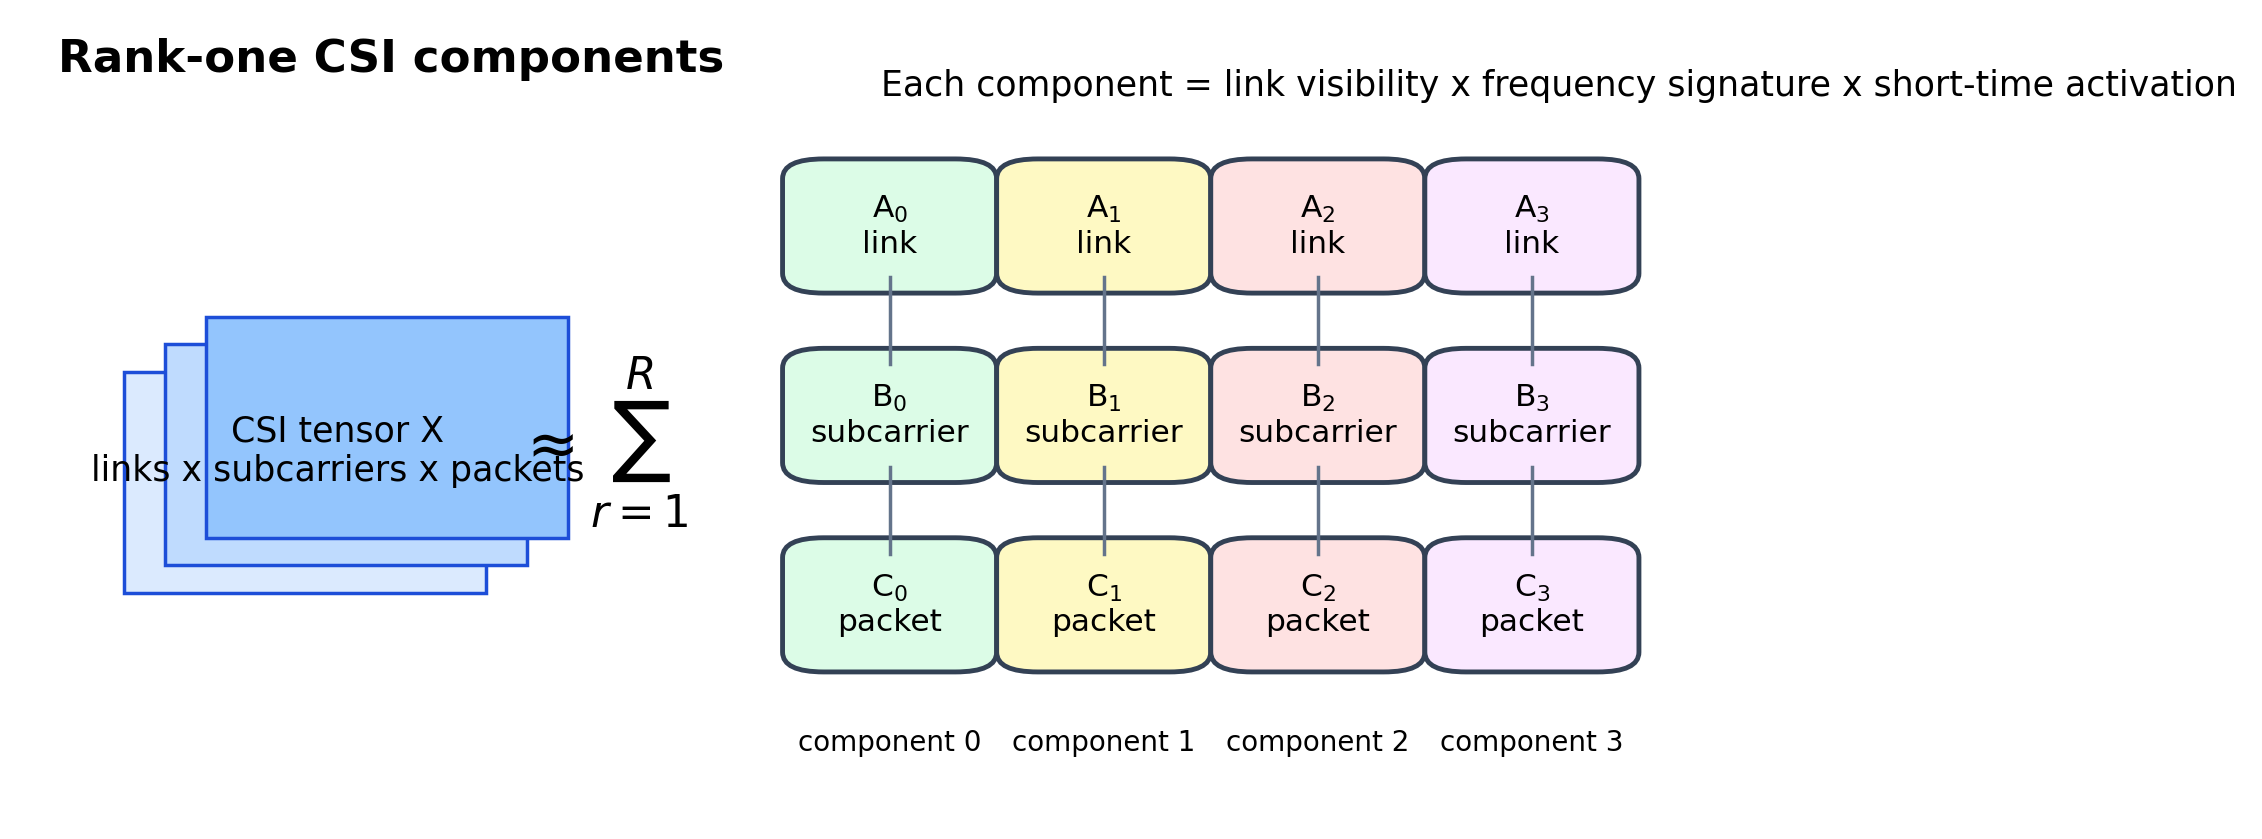
\includegraphics[width=\linewidth]{figures/fig2_decomposition.pdf}
\caption{Rank-one component view of CSI. Each component has a link factor, subcarrier factor, and packet factor.}
\label{fig:decomposition}
\end{figure}

\subsection{Optimization}

The basic reconstruction objective is
\begin{equation}
\mathcal{L}_{rec}=\|X-\hat{X}\|_F^2.
\end{equation}
More generally, CSI decomposition can be written as a constrained objective:
\begin{equation}
\min_{A,B,C,G_\omega}
\mathcal{L}_{pose}(G_\omega(z),y)
+\lambda_r\|X-\hat{X}\|_F^2
+\lambda_d\mathcal{L}_{div}
+\lambda_s\mathcal{L}_{sparse}
+\lambda_t\mathcal{L}_{smooth}
\end{equation}
\begin{equation}
\text{s.t.}\quad A\ge0,\;B\ge0,\;C\ge0,\qquad
z=[A(:),B(:),C(:)].
\end{equation}
Here $\mathcal{L}_{pose}$ makes components useful for HPE, $\mathcal{L}_{div}$ discourages redundant components, $\mathcal{L}_{sparse}$ sharpens component support, and $\mathcal{L}_{smooth}$ stabilizes temporal activations. The current experiments use the unsupervised case $\lambda_d=\lambda_s=\lambda_t=0$ and train $G_\omega$ after decomposition. This is intentionally conservative: if unsupervised CP already helps tiny regressors, then supervised or constrained decomposition has a clear path to improve.

For the unsupervised CP solver, we use multiplicative updates. Let $X_{(1)}$, $X_{(2)}$, and $X_{(3)}$ denote mode unfoldings, $\odot$ the Khatri-Rao product, and $\circ$ elementwise multiplication. The updates are:
\begin{align}
A &\leftarrow A\circ
\frac{X_{(1)}(B\odot C)}
{A((B^TB)\circ(C^TC))+\epsilon},\\
B &\leftarrow B\circ
\frac{X_{(2)}(A\odot C)}
{B((A^TA)\circ(C^TC))+\epsilon},\\
C &\leftarrow C\circ
\frac{X_{(3)}(A\odot B)}
{C((A^TA)\circ(B^TB))+\epsilon}.
\end{align}
Factors are normalized after update cycles to control scale ambiguity.

\subsection{Compact Pose Features}

The decomposed feature is
\begin{equation}
z=[A(:),B(:),C(:)].
\end{equation}
For rank $R=4$, MM-Fi frames are reduced from $3\times114\times10=3420$ raw values to
\begin{equation}
4(3+114+10)=508
\end{equation}
component values. This gives a $6.73\times$ smaller representation.

This compactness is not only a storage benefit. It changes the statistical problem faced by the regressor. The raw frame mixes modes multiplicatively and forces the model to infer interactions among links, subcarriers, and packets. The CP feature explicitly separates these modes, giving the regressor structured summaries.

\subsection{Tiny Pose Regressors}

We train lightweight regressors from $z$ to the 51-dimensional 3D keypoint vector. We evaluate Ridge regression, partial least squares (PLS), a one-hidden-layer MLP with 64 units, and ExtraTrees. The regressors are intentionally simple. If componentized CSI is meaningful, pose prediction should not require a heavy neural network.

Each regressor answers a different question. Ridge tests whether the relationship between component features and pose is close to linear. PLS tests whether a low-dimensional latent linear relationship exists between factors and pose. MLP64 tests whether a very small neural model benefits from mild nonlinearity. ExtraTrees tests whether decomposed features contain nonlinear pose structure accessible to classical ML.

\textbf{Plug-and-play predictor view.}
The regressor is not the main contribution. It is a replaceable module:
\begin{equation}
\hat{y}=G_\omega(z),\qquad
G_\omega\in\{\text{Ridge},\text{PLS},\text{MLP},\text{CNN},\text{Transformer},\text{Tree Ensemble}\}.
\end{equation}
This plug-and-play design is important. A cloud setting may use a larger Transformer or graph decoder on decomposed features. An edge setting may use Ridge, decision trees, or a one-hidden-layer MLP. The decomposition front-end stays the same and provides structured, compact input to whichever predictor is appropriate for the hardware budget. Thus, \method\ should be read as a decomposition framework rather than a specific tiny regressor.

\subsection{Component Quality Evaluation}

Since decomposition is the main contribution, downstream PCK alone is insufficient. We evaluate components by:
\begin{itemize}
    \item reconstruction error $\|X-\hat{X}\|_F/\|X\|_F$;
    \item feature compactness relative to raw CSI;
    \item component ablation by removing one rank-one component;
    \item factor-mode ablation by removing $A$, $B$, or $C$;
    \item factor importance from the downstream regressor;
    \item factor correlations as a measure of separation.
\end{itemize}

\section{Experiments}

\subsection{Dataset and Protocol}

We evaluate on MM-Fi using the frame-level protocol used by HPE-Li. Each input is one CSI frame and each target is one pose label. We follow protocol3 and the HPE-Li random subject split logic. PCK is computed using the HPE-Li metric: 2D keypoint error is normalized by the torso scale between keypoints 1 and 11.

The full local MM-Fi download contains all $320{,}760$ expected frame-level Wi-Fi CSI samples. The reproduced HPE-Li protocol-3 split gives $224{,}532$ training frames and $96{,}228$ validation/test frames. Following the HPE-Li evaluation code, we split the validation side into validation and test halves, giving $48{,}114$ held-out test frames for the reported results.

\subsection{Baselines}

We compare mean pose, raw CSI statistics with ML regressors, CP components with the same regressors, and the reported HPE-Li result. Raw statistics summarize the raw frame over links, subcarriers, and packets. CP components use the factor vector $z$.

\textbf{Mean pose.}
Mean pose ignores CSI and predicts the average training pose. It is a sanity check. If a method cannot beat mean pose, the representation is not useful.

\textbf{Raw statistics.}
Raw statistics summarize the CSI frame by means and standard deviations across modes. This baseline is intentionally simple but strong: it tests whether the dataset can be solved by coarse frequency/link statistics without decomposition.

\textbf{CP components.}
CP components use factorized CSI features. Comparing raw statistics and CP components under the same regressors isolates the value of decomposition.

\textbf{HPE-Li reference.}
HPE-Li is included as an external reported reference because it is a strong lightweight Wi-Fi HPE method. We use the same MM-Fi frame-level protocol and the same PCK implementation for metric compatibility.

\subsection{SOTA Landscape and Comparison Scope}

Table~\ref{tab:sota_scope} summarizes representative Wi-Fi HPE systems and the comparison status. Wi-Fi HPE papers do not all report the same dataset, split, keypoint definition, or metric. Therefore, we separate direct comparison from contextual comparison. HPE-Li is the strongest direct reference because it uses MM-Fi, frame-level CSI, protocol3, and the same PCK implementation. Other methods such as MetaFi, Wi-Mose, GoPose, GraphPose-Fi, and C-MambaPose establish the broader SOTA landscape, but their reported numbers are not always protocol-compatible with HPE-Li/MM-Fi protocol3.

\begin{table*}[t]
\centering
\caption{Wi-Fi HPE comparison scope. ``Direct'' means the result is comparable under the MM-Fi frame-level PCK protocol used in this paper.}
\label{tab:sota_scope}
\begin{tabular}{lccccp{4.8cm}}
\toprule
Method & Dataset / split & Direct? & Params & FLOPs & Notes \\
\midrule
Person-in-WiFi & custom & No & -- & -- & Early fine-grained Wi-Fi person perception; not MM-Fi protocol3. \\
Wi-Mose & custom & No & -- & -- & Reports distance-error metrics such as P-MPJPE rather than HPE-Li PCK. \\
GoPose & custom & No & -- & -- & Uses reflected Wi-Fi and spatial spectrum; reports cm-level pose accuracy. \\
MetaFi / MetaFi++ & custom / MM-Fi & Partial & up to 26.52M & -- & Strong neural Wi-Fi HPE family; exact protocol3 PCK must be reproduced for fair comparison. \\
GraphPose-Fi & MM-Fi & Partial & -- & -- & Reports MM-Fi PCK on protocol settings, but not the exact HPE-Li frame-level protocol used here. \\
C-MambaPose & MM-Fi & Partial & 3.78M & -- & Recent complex-valued Mamba/GNN model for cross-environment MM-Fi pose. \\
HPE-Li & MM-Fi protocol3 & Yes & 1.66M & 2.42G & Strong lightweight direct baseline. \\
\method\ CP+MLP64 & MM-Fi protocol3 & Yes & 35.9K & 1.00M & Deployable decomposition-first model. \\
\method\ CP+ExtraTrees & MM-Fi protocol3 & Yes & large & -- & Accuracy upper bound for classical ML, not the tiny deployment model. \\
\bottomrule
\end{tabular}
\end{table*}

\subsection{Implementation}

Each CSI frame is loaded from its MM-Fi MATLAB file, invalid values are replaced, and the frame is min-max normalized. Rank is set to $R=4$. ExtraTrees uses 80 trees, maximum depth 24, and minimum leaf size 4. We do not tune aggressively; the goal is to test feasibility and component usefulness.

\section{Results}

\subsection{Main Accuracy}

Table~\ref{tab:main} reports the main results on full MM-Fi. CP components improve over raw statistics under the lightweight MLP64 and under ExtraTrees, showing that decomposition provides useful structure beyond coarse frame statistics.

\begin{table*}[t]
\centering
\caption{Frame-level MM-Fi protocol-3 results on the full dataset.}
\label{tab:main}
\begin{tabular}{lrrrrrr}
\toprule
Method & PCK$_{50}$ & PCK$_{40}$ & PCK$_{30}$ & PCK$_{20}$ & PCK$_{10}$ & MPJPE \\
\midrule
Mean pose & 73.10 & 62.36 & 46.92 & 27.45 & 9.51 & 0.246 \\
Raw stats + Ridge & 80.12 & 71.17 & 58.14 & 39.06 & 14.52 & 0.219 \\
Raw stats + MLP64 & 82.14 & 74.74 & 63.43 & 44.69 & 17.37 & 0.208 \\
Raw stats + ExtraTrees & 81.99 & 74.38 & 63.68 & 47.27 & 21.22 & 0.204 \\
CP components + Ridge & 78.91 & 69.96 & 56.99 & 38.18 & 14.18 & 0.223 \\
CP components + PLS16 & 77.87 & 68.42 & 55.21 & 36.59 & 13.25 & 0.227 \\
CP components + MLP64 & 82.37 & 75.09 & 64.13 & 46.24 & 18.37 & 0.209 \\
CP components + ExtraTrees & \textbf{83.32} & \textbf{76.34} & \textbf{66.20} & \textbf{50.40} & \textbf{24.01} & \textbf{0.197} \\
HPE-Li reported & 85.12 & 78.18 & 68.22 & 52.07 & -- & -- \\
\bottomrule
\end{tabular}
\end{table*}

The result supports the decomposition-first hypothesis, but it also gives a sober boundary. Vanilla unsupervised CP does not yet surpass HPE-Li accuracy on full MM-Fi. However, it consistently improves lightweight nonlinear regressors over raw-statistic features: CP+MLP64 improves PCK$_{20}$ by 1.54 points, and CP+ExtraTrees improves PCK$_{20}$ by 3.13 points. This suggests that decomposition is useful, while also motivating constrained and pose-aware decomposition as the next step.

\begin{figure*}[t]
\centering
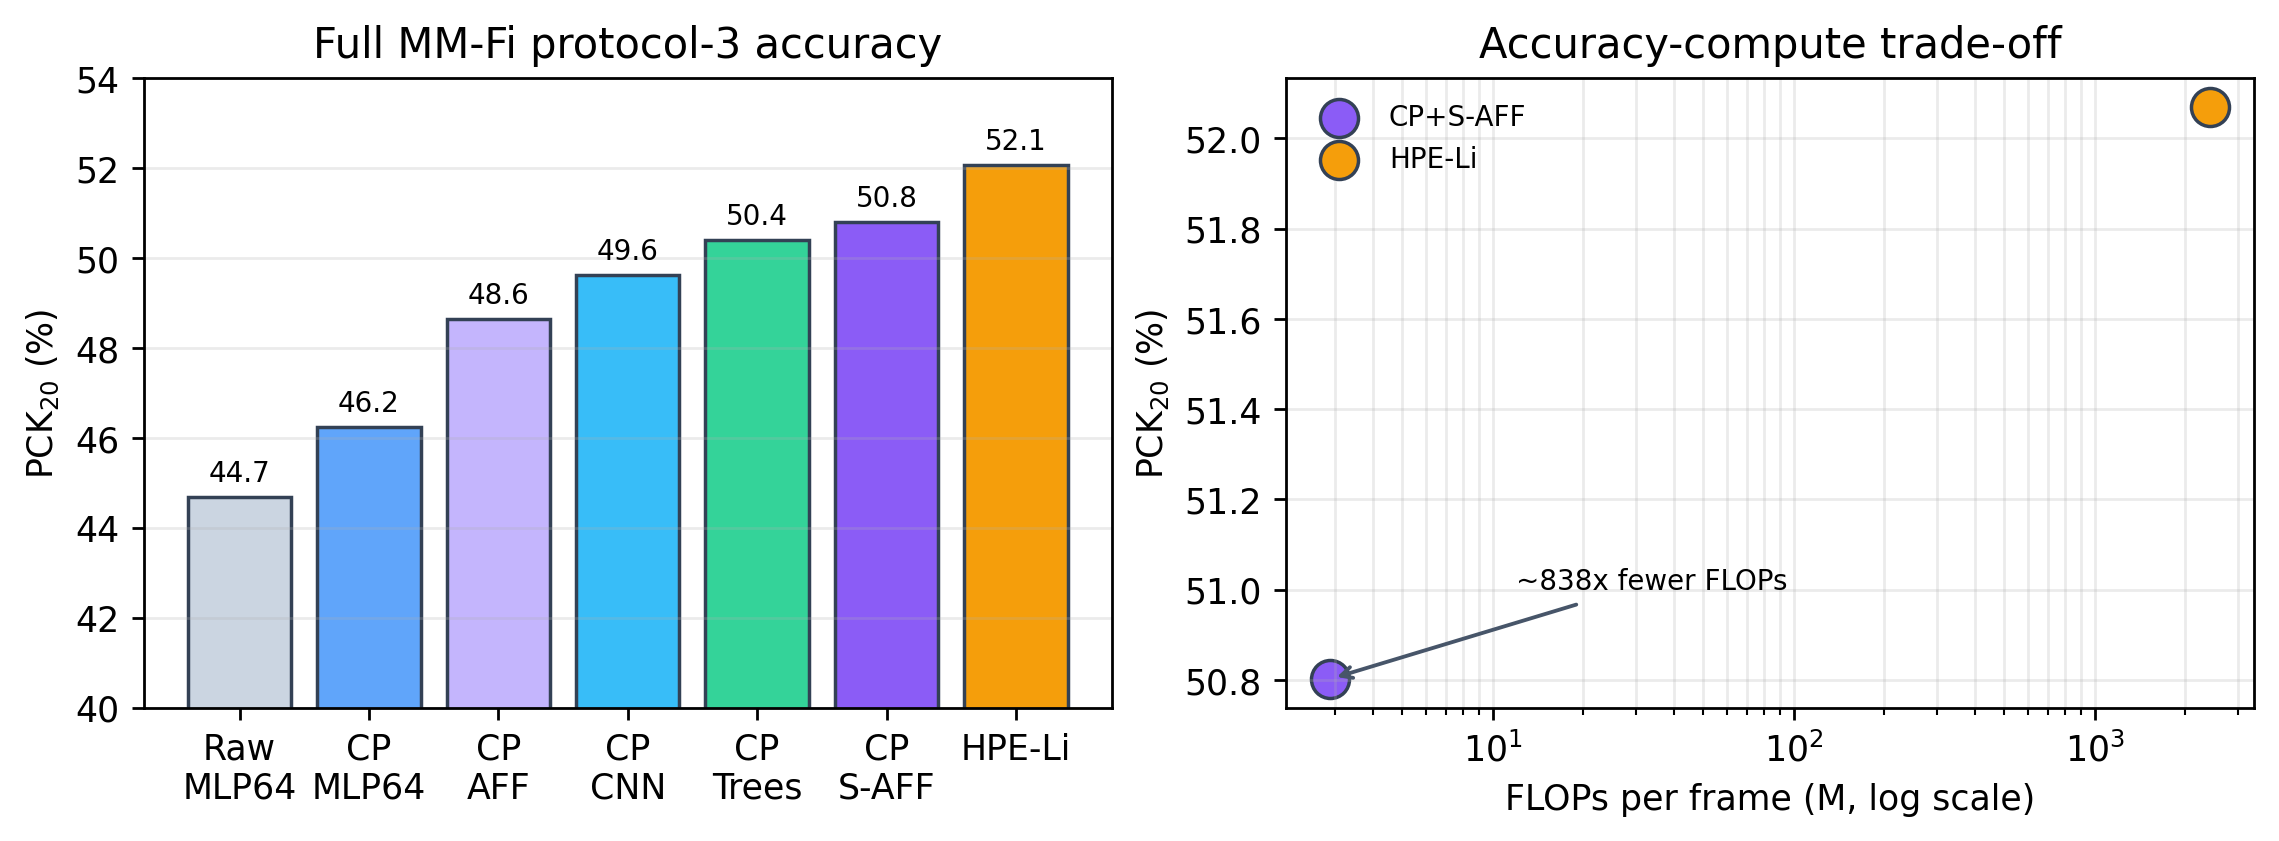
\includegraphics[width=0.86\linewidth]{figures/fig6_full_results_complexity.pdf}
\caption{Full MM-Fi accuracy and complexity trade-off. CP components improve lightweight predictors over raw statistics, while CP+MLP64 uses orders of magnitude fewer FLOPs than HPE-Li.}
\label{fig:full_results_complexity}
\end{figure*}

\subsection{RQ1: Do Compact Components Retain Pose Information?}

Yes. CP components reduce the feature dimension by $6.73\times$ yet retain enough information for competitive HPE. CP components improve over raw statistics when the downstream regressor is nonlinear, including both MLP64 and ExtraTrees. This suggests that factorization preserves task-relevant structure rather than merely compressing away pose information.

The result is especially notable because CP is unsupervised in this experiment. The decomposition is not optimized with pose labels; it only reconstructs the CSI frame. If unsupervised components already perform well, pose-aware decomposition has room to improve.

\subsection{RQ2: Can Tiny ML Approach Neural HPE?}

The current answer is partially yes. CP+MLP64 does not match HPE-Li accuracy, but it uses only 35.9K parameters and about 1.00M FLOPs per frame, compared with HPE-Li's reported 1.66M parameters and 2.42G FLOPs. This is approximately 46$\times$ fewer parameters and over 2400$\times$ fewer FLOPs. CP+ExtraTrees reaches closer accuracy but is not the preferred deployment model because the tree ensemble is much larger. The key message is therefore not that vanilla CP already wins all accuracy metrics, but that decomposition makes extremely small predictors viable.

\subsection{Component Pose Relevance}

We train ExtraTrees on all CP components and remove one component at test time. Figure~\ref{fig:component_ablation} and Table~\ref{tab:component} show that every component matters.

\begin{figure}[t]
\centering
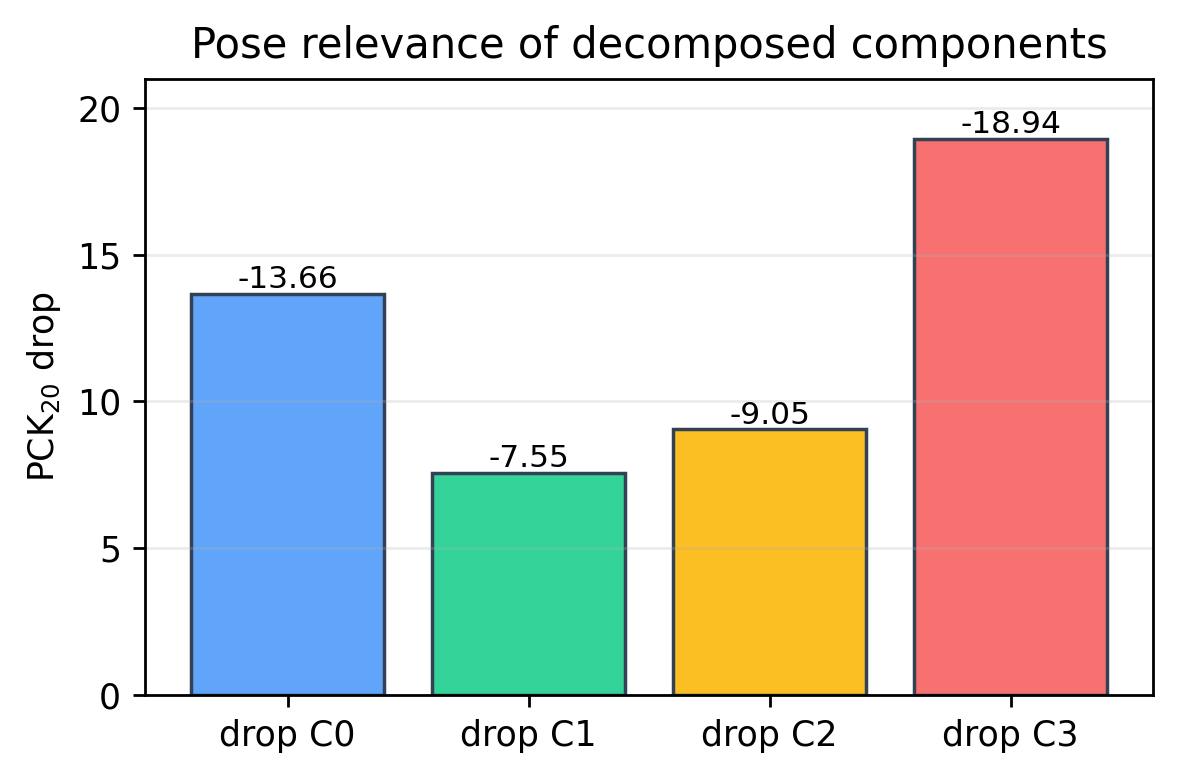
\includegraphics[width=\linewidth]{figures/fig3_component_ablation.pdf}
\caption{Component pose relevance. Removing any component reduces PCK$_{20}$, showing that the decomposition is not cosmetic.}
\label{fig:component_ablation}
\end{figure}

\begin{table}[t]
\centering
\caption{Component ablation with CP components + ExtraTrees.}
\label{tab:component}
\begin{tabular}{lrr}
\toprule
Input & PCK$_{20}$ & Drop \\
\midrule
All components & 50.40 & 0.00 \\
Drop component 0 & 36.74 & -13.66 \\
Drop component 1 & 42.85 & -7.55 \\
Drop component 2 & 41.35 & -9.05 \\
Drop component 3 & 31.46 & -18.94 \\
\bottomrule
\end{tabular}
\end{table}

This is the key evidence for our thesis. If decomposition were merely compression, dropping one component would have little effect. Instead, every component contributes to pose prediction, and the most important component accounts for 18.94 PCK$_{20}$ points.

\subsection{RQ3: Are Components Pose-Relevant?}

Yes. Table~\ref{tab:component} directly answers this question. Dropping any component hurts PCK$_{20}$. The drops are not tiny: they range from 7.55 to 18.94 points. This means the downstream model uses multiple decomposed factors, and the components carry distinct pose-relevant information.

The corresponding ``only component'' experiment, stored in the output artifacts, shows that no single component is sufficient. Each isolated component performs close to the mean-pose baseline, while all components together achieve much higher accuracy. This indicates that pose estimation depends on a combination of latent CSI modes.

\subsection{Which Physical Mode Matters?}

We remove entire factor modes from the CP feature vector. Figure~\ref{fig:factor_importance} shows the result. The subcarrier factor $B$ dominates the current frame-level setting. Removing $B$ causes a 24.90-point PCK$_{20}$ drop, while removing link factor $A$ causes a 2.68-point drop and removing packet factor $C$ causes only a 0.26-point drop.

\begin{figure}[t]
\centering
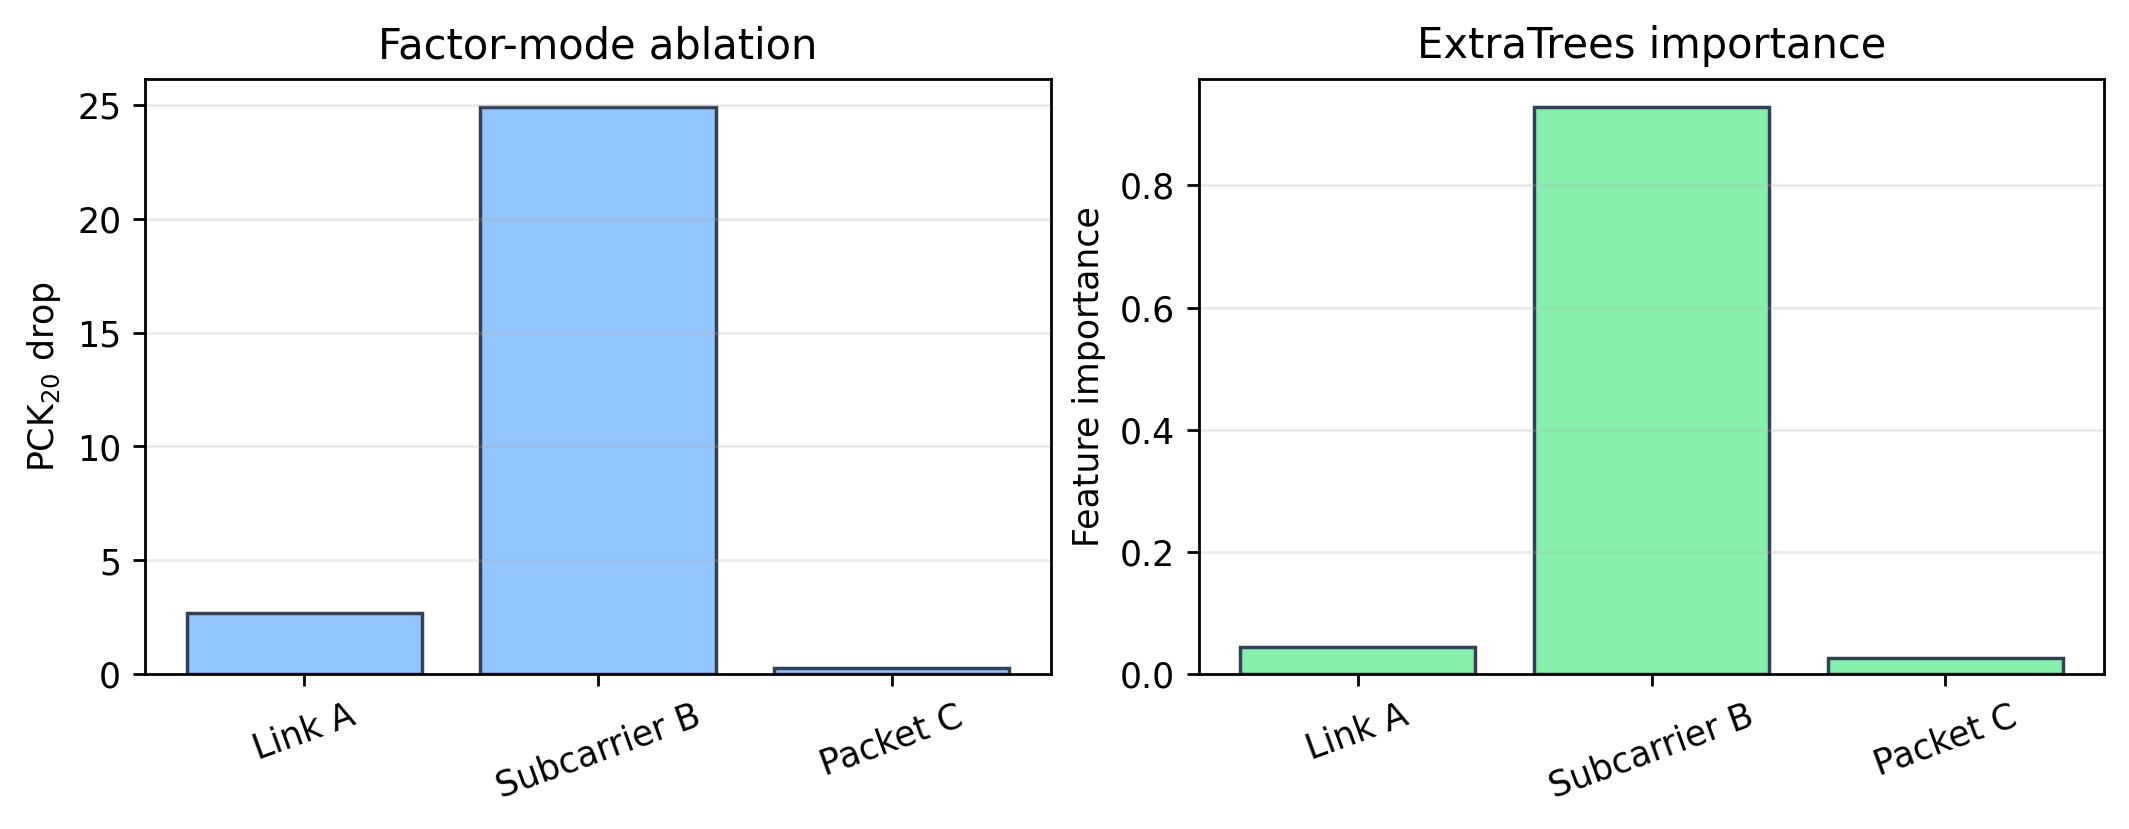
\includegraphics[width=\linewidth]{figures/fig4_factor_importance.pdf}
\caption{Factor-mode analysis. Under single-frame MM-Fi, the subcarrier factor carries most pose-relevant information.}
\label{fig:factor_importance}
\end{figure}

This makes physical sense. A single MM-Fi frame contains only 10 packets, which limits temporal motion evidence. The subcarrier factor captures frequency-selective multipath structure and is therefore the strongest pose carrier. A temporal-window version should expose stronger Doppler and time factors, but it must be compared fairly by giving all baselines the same temporal context.

\subsection{Why the Subcarrier Factor Dominates}

The dominance of $B$ is informative. In one frame, there is little temporal evidence; the packet axis has only ten samples. The subcarrier axis has 114 values and captures fine-grained frequency selectivity. Since frequency selectivity is shaped by multipath geometry, it can encode pose-dependent body-channel interactions. This suggests that frame-level Wi-Fi HPE may rely more on instantaneous multipath signatures than on within-frame motion.

This observation gives a stronger story than a black-box accuracy table. It identifies which physical mode matters under the HPE-Li protocol and motivates a separate temporal-window study for Doppler-aware decomposition.

\subsection{Efficiency}

Table~\ref{tab:complexity} reports the parameter and compute cost of the lightweight \method\ variants. The rank-4 CP representation reduces each frame from 3420 raw CSI values to 508 component features. The Ridge and MLP64 heads contain only 25.9K and 35.9K trainable parameters, respectively. When CP extraction is included, a 10-iteration CP+MLP64 pipeline requires approximately 1.00M FLOPs per frame. A 5-iteration version reduces the full pipeline to 0.54M FLOPs.

\begin{table}[t]
\centering
\caption{Model complexity of lightweight \method\ variants. FLOPs include CP feature extraction and pose regression.}
\label{tab:complexity}
\begin{tabular}{lrrrr}
\toprule
Model & Params & CP iters & MACs & FLOPs \\
\midrule
CP+Ridge & 25.9K & 5 & 0.259M & 0.518M \\
CP+MLP64 & 35.9K & 5 & 0.269M & 0.538M \\
CP+Ridge & 25.9K & 10 & 0.492M & 0.984M \\
CP+MLP64 & 35.9K & 10 & 0.502M & 1.004M \\
CP+Ridge & 25.9K & 35 & 1.658M & 3.316M \\
CP+MLP64 & 35.9K & 35 & 1.668M & 3.336M \\
\bottomrule
\end{tabular}
\end{table}

These numbers support the edge-device argument, but they also clarify the current trade-off. ExtraTrees gives the best accuracy in Table~\ref{tab:main}, but its serialized model is large and should be treated as an accuracy upper bound for classical ML. The deployable version is CP+MLP64 or CP+Ridge: both are tiny, have sub-megabyte model storage, and require roughly one million FLOPs per frame with 10 CP iterations. Prediction is fast once features are extracted; in our Python implementation, Ridge and MLP inference take microseconds per sample. The main deployment bottleneck is therefore decomposition extraction, not pose regression. A future deployment version should replace iterative CP with a learned dictionary or feed-forward non-negative factor extractor.

\subsection{Component Quality}

On 3,000 sampled frames, rank-4 CP achieves mean reconstruction error $0.0863$, indicating good CSI reconstruction. However, factor correlations remain high: link factor correlation is $0.6973$, subcarrier factor correlation is $0.3832$, and packet factor correlation is $0.5921$. Vanilla CP is predictive, but not physically clean enough to claim true source separation. This motivates constrained pose-aware decomposition.

\section{Discussion}

\textbf{What this proves.}
The current evidence proves that decomposed CSI components are compact, predictive, and pose-relevant on the full MM-Fi frame-level protocol. Vanilla CP does not yet beat HPE-Li accuracy, but it improves lightweight nonlinear regressors over raw statistics and reduces the deployable model to tens of thousands of parameters.

\textbf{What remains open.}
We do not yet claim that vanilla CP recovers clean physical human-motion sources. The factor correlations are too high. We also do not claim that unsupervised CP is the final model; the next version needs constrained and pose-aware decomposition to close the remaining accuracy gap to HPE-Li.

\textbf{Next technical step.}
The final method should use constrained, pose-aware decomposition:
\begin{equation}
\mathcal{L}=
\mathcal{L}_{rec}
\lambda_{pose}\mathcal{L}_{pose}
\lambda_{div}\mathcal{L}_{div}
\lambda_s\mathcal{L}_{sparse}
\lambda_t\mathcal{L}_{smooth}.
\end{equation}
Diversity can reduce redundant components, sparsity can sharpen link/frequency factors, smoothness can stabilize temporal activations, and pose supervision can make factors more keypoint-relevant.

\section{Conclusion}

This paper introduces \method, a decomposition-first framework for Wi-Fi human pose estimation. The central message is that complicated CSI should be decomposed into physically meaningful components before being passed to a learning model. On the full MM-Fi frame-level protocol, compact CP components improve lightweight nonlinear regressors over raw-statistic features and component ablation confirms that the factors are strongly pose-relevant. These findings support a practical research direction: build Wi-Fi HPE systems around interpretable signal decomposition, then use tiny predictors for deployment.

\bibliographystyle{aaai}
\begin{thebibliography}{99}

\bibitem{personwifi2019}
F. Wang et al.
\newblock Person-in-WiFi: Fine-grained person perception using WiFi.
\newblock arXiv:1904.00276, 2019.

\bibitem{wimose2020}
Y. Wang et al.
\newblock From point to space: 3D moving human pose estimation using commodity WiFi.
\newblock arXiv:2012.14066, 2020.

\bibitem{gopose2022}
Y. Ren and J. Yang.
\newblock 3D human pose estimation for free-form and moving activities using WiFi.
\newblock arXiv:2204.07878, 2022.

\bibitem{mmfi2023}
J. Yang et al.
\newblock MM-Fi: Multi-modal non-intrusive 4D human dataset for versatile wireless sensing.
\newblock arXiv:2305.10345, 2023.

\bibitem{hpeli2024}
T. D. Gian, T. D. Lai, T. V. Luong, K.-S. Wong, and V.-D. Nguyen.
\newblock HPE-Li: WiFi-enabled lightweight dual selective kernel convolution for human pose estimation.
\newblock In \emph{ECCV}, 2024.

\bibitem{efficientfi2022}
J. Yang, X. Chen, H. Zou, D. Wang, Q. Xu, and L. Xie.
\newblock EfficientFi: Towards large-scale lightweight WiFi sensing via CSI compression.
\newblock arXiv:2204.04138, 2022.

\bibitem{sensefi2022}
J. Yang, X. Chen, D. Wang, H. Zou, C. X. Lu, S. Sun, and L. Xie.
\newblock SenseFi: A library and benchmark on deep-learning-empowered WiFi human sensing.
\newblock arXiv:2207.07859, 2022.

\bibitem{litehar2022}
H. Salehinejad and S. Valaee.
\newblock LiteHAR: Lightweight human activity recognition from WiFi signals with random convolution kernels.
\newblock arXiv:2201.09310, 2022.

\bibitem{factorhar2023}
J. Liu et al.
\newblock A Wi-Fi signal-based human activity recognition using high-dimensional factor models.
\newblock arXiv:2311.05921, 2023.

\bibitem{widefus2026}
X. Chen, C. Li, W. Meng, and W. Xiao.
\newblock WiDeFus: A Wi-Fi-based lightweight human activity recognition via CSI component decomposition and adaptive feature fusion.
\newblock \emph{IEEE Transactions on Cognitive Communications and Networking}, 2026.

\bibitem{kolda2009}
T. G. Kolda and B. W. Bader.
\newblock Tensor decompositions and applications.
\newblock \emph{SIAM Review}, 2009.

\bibitem{lee1999}
D. D. Lee and H. S. Seung.
\newblock Learning the parts of objects by non-negative matrix factorization.
\newblock \emph{Nature}, 1999.

\end{thebibliography}

\end{document}
